\chapter{Poincare map}
\newcommand{\dpmap}{\mathcal{D}\mathcal{P}}
\newcommand{\pmap}{\mathcal{P}}
\newcommand{\nfp}{n_\text{fp}}
\newcommand{\z}{z}

In the study of continuous dynamical systems, it is often convenient to consider a discrete map defined by the intersection of the trajectories with a lower-dimensional subspace and which captures some properties of the continuous case. In the case of particles following the magnetic field of a toroidal apparatus, the intersection of their trajectories with a constant $\phi$ cross-section reveals the distinct region of different field line behaviour~: closed surfaces, islands, chaotic regions, and is known as a \textit{Poincare} section.

\begin{figure}[h!]
    \subfloat[W7-X]{%
        \includegraphics[width=0.3\textwidth]{example-image-a}
    }
    \hfill
    \subfloat[NCSX]{%
        \includegraphics[width=0.3\textwidth]{example-image-b}
    }
    \hfill
    \subfloat[LHD]{%
        \includegraphics[width=0.3\textwidth]{example-image-c}
    }
    \caption{[w7x and other stell poincare section]}
\end{figure}
[
See for instance 
in experiments using fluorencent rod one can find this.
]

To compute a Poincare section numerically, the field line need to be traced and the crossings recorded. The evolution of a particle along the magnetic field $\textbf{B}$ will be described in cylindrical coordinates. By taking into account only the center of the gyro-motion.

In fact it is a map defined by looking at the flow of vector field.

\noindent
\makebox[\textwidth]{%
  \begin{tcolorbox}[colback=lightgray!10, colframe=black, width=0.85\textwidth, boxrule=0.5mm, sharp corners]
    \textbf{Geometric consideration} : Throughout this document, the convention adpoted is that of the contravariant component for vectors. That is, for example, $\textbf{B}$ in cylindrical coordinates has the form $B^R = \textbf{B}\cdot\nabla R$, $B^\phi = \textbf{B}\cdot\nabla\phi$ and $B^Z = \textbf{B}\cdot\nabla Z$. In the formalism of differential geometry, one writes $B=B^i\partial_i$. The basis $\{\partial_i\}_i$ is orthogonal and holonomic but the element may not be unitary, as for $\partial_\phi$. On the other hand, the component in the common orthonormal basis $e_i$ will be written with subscript as $\tilde{B}^i$. [SEE APP]
  \end{tcolorbox}
}

The trajectory curve $\gamma : \mathbb{R}\rightarrow\mathbb{R}^+\times[0,2\pi[\times\mathbb{R} \eqqcolon \mathcal{M}$, $t \mapsto \gamma(t) = (R(t),\,\phi(t),\,Z(t))$ we are interested in is such that the tangent vector at each point is given by $\dot{\gamma}(t)= \textbf{B} = B^i\partial_i \in T_{\gamma(t)}\mathcal{M}$. Specifying the initial point $\gamma(0) = \textbf{x}_0$ identifies a specific curve~:
\begin{align*}
    \gamma(t) = \int_0^t\dot{\gamma}(s)ds + \textbf{x}_0 \quad \text{with} \quad   \dot{\gamma}^i(t)= (\frac{dR}{dt},\,\frac{d\phi}{dt},\,\frac{dZ}{dt}) = (B^R, B^\phi, B^Z).
\end{align*}
Provided that the sign of $B^\phi(R, \phi, Z)$ is either positive or negative on $\gamma$, $B^\phi$ is never zero, the map~:
\begin{equation*}
    t(\phi) = \int \frac{dt}{d\phi}d\phi = \int_0^\phi \frac{1}{B^\phi}d\phi
\end{equation*}

defines a handy change of variable for which the $\phi$ evolution is linear. Indeed $\gamma$ can be re-parameterized as $\phi \mapsto \gamma(\phi) = (R(\phi),\,\phi,\,Z(\phi))$ with~$\dot{\gamma}$~:
\begin{equation*}
    \dot{\gamma}^i(\phi) = (\frac{dR}{d\phi},\,1,\,\frac{dZ}{d\phi}) = (\frac{dR}{dt}\frac{dt}{d\phi},\,1,\,\frac{dZ}{dt}\frac{dt}{d\phi}) = (B^R/B^\phi,\, 1,\,B^Z/B^\phi).
\end{equation*}
Due to the choice of coordinates the field will have at most a $\phi$ periodicity of $2\pi$, yet in stellarator configurations have azymuthal redundancy. Their period is $T = 2\pi/n_\text{fp}$ where $n_\text{fp}\in\mathbb{N}^\star$ is the number of field period in a complete toroidal rotation. For example, W7X and LHD have 5 and 10 field periods respectively. If the field is not periodic then $n_\text{fp} = 1$ and, in contrast, for an axisymmetric device without defaults $n_\text{fp} = +\infty$, the case of ideal Tokamaks.

The Poincare section is hence identical for $\phi_i$ and $\phi_i+kT$, $k\in\mathbb{Z}$. Writing $\Omega$ the set of initial points in the $\phi_i$ plane for which $\gamma$ is effectively re-parametrizable between $\phi_i$ and $\phi_i + T$, allows to define the map $\pmap : \Omega \rightarrow \mathbb{R}_+\times\mathbb{R}$ as~:
\begin{equation*}
    (\tilde{R},\tilde{Z}) \mapsto \pmap(\tilde{R},\tilde{Z}) = \int_{\phi_i}^{\phi_i+T}(
        \dot{\gamma}^R(s),\,
        \dot{\gamma}^Z(s)
    )\,ds + (\tilde{R},\tilde{Z})
\end{equation*}
with $\textbf{x}_0 = (\tilde{R},\,\phi_i,\,\tilde{Z})$. \figref{fig:th-poincare-map} represent an hypothetical $\nfp = 3$ configuration where an initial starting point $z_0\coloneqq (\tilde{R}_i,\tilde{Z}_i)$ gets map to the $\phi_i + T$ cross section. The evolution of the intersection for $z_0$ is then simply $z_{i+1} = \pmap(z_i)$ and $z_n = \pmap^n(z_0)$. 

\begin{figure}[H]
    \centering
    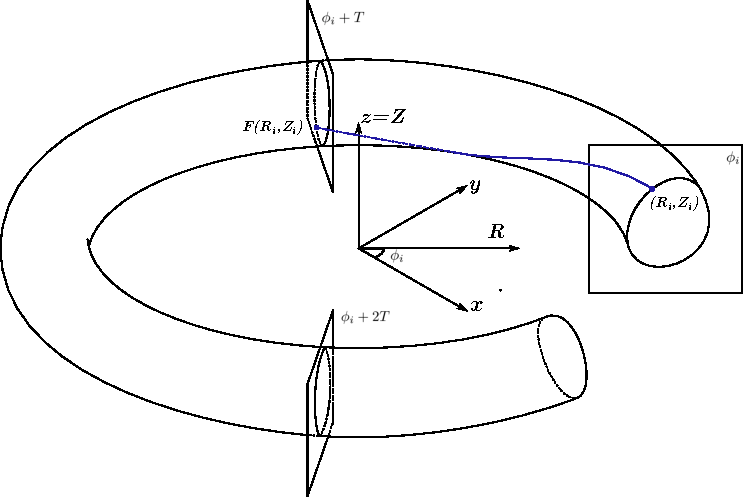
\includegraphics{images/theory/poincare-torus.pdf}
    \caption{Trajectory of a particle in a toroidal device (Tokamak/Stellarator) from a starting point $(\tilde{R}, \tilde{Z})$ in a $\phi = \phi_i$ section to a point in the $\phi = \phi_i + T$ plane with $T$ the azymuthal periodicity of the magnetic field.}
    \label{fig:th-poincare-map}
\end{figure}

As the evolution is performed by following $\mathbf{B}$ and due to the magnetic field been divergence free $\nabla\cdot\textbf{B} = 0$, the flux through any surface obtained by mapping a simple path in $\phi_i$ to $\phi_i + T$ will be zero. This result in the key property of $\pmap$ being flux-conserving ; the flux through any closed surface $\Sigma \subset \Omega$ is equal to the one through $\pmap(\Sigma)$~:
\begin{equation*}
    \iint\limits_{\Sigma}\textbf{B}\cdot\textbf{dS} = \iint\limits_{\pmap(\Sigma)}\textbf{B}\cdot\textbf{dS}.
\end{equation*}
The determinant of the Jacobian matrix for a general flow $\Phi(x_0, t)$ of a vector field $v$, which does not depend on time, is related to the divergence of $v$ \cite[p.408]{hirsch_differential_2013} by~:
\begin{equation}\label{eq:det-div-flow}
    \text{det}(\mathcal{D}\Phi(x_0, t)) = \text{det}(\mathcal{D}\Phi(x_0, 0))\exp\left(\int_0^t\text{Tr}(\nabla v(s)) ds\right) = \exp\left(\int_0^t \nabla\cdot v(s) ds\right)
\end{equation}
with $v(\Phi(x_0, s))$ written implicitly as $v(s)$. In the case of the flow in cylindrical coordinates, \citeauthor{wei_invariant_2023} use \equref{eq:det-div-flow} to derive the relation~(Eq.8):
\begin{equation*}\label{eq:det-div-pmap}
    \text{det}(\mathcal{D}\Phi(x_0, \phi_i, \phi_e)) = \exp\left(\int_{\phi_i}^{\phi_e} \frac{R\,(\nabla\cdot v)}{\tilde{v}^\phi} ds\right)\frac{\tilde{v}^\phi(\phi_i)}{\tilde{v}^\phi(\phi_e)}.
\end{equation*}
It gives for the determinant of $\dpmap \in \mathbb{R}^{2\times2}$ that~:
\begin{equation}\label{eq:pmap-det}
    \text{det}(\dpmap(\tilde{R}, \tilde{Z})) = B^\phi(\tilde{R},\phi_i, \tilde{Z})/B^\phi(\pmap^{\tilde{R}}(\tilde{R},\tilde{Z}), \phi_i+T,\pmap^{\tilde{Z}}(\tilde{R},\tilde{Z})).
\end{equation}
The last identity may also be recovered more directly using differential forms as in \cite{meiss_thirty_2015}, the derivation is given in \appref{forms}.

\section{Fixed points}
Periodic orbit of the Poincaré map $\pmap$ are particularly important as they define field line that are close. A fixed point $\z^\star\in\Omega$ of order $k$ for $\pmap$ is such that $\pmap^k(\z^\star) = \z^\star$. 

In the case of an island or island chain, the surface on which they happen (under resonable condition you can have them [CITE]), the number of winding that a field line starting on that surface does around the magnetic axis is given by the rotational transform $\iota$ over 2pi and is equal to $n/m$. It means that initial fixed point $x^\star$ evolves and after $m$ toroidal turns it will come back to itself, having perform n poloidal turns. We can see then that the number of intersections will be equal to $m$. the order of this fixed point for the poincare map is then at max $k=m\nfp$.

\begin{figure}[H]
    \subfloat[5/5 island in]{%
        \includegraphics[width=0.5\textwidth]{example-image-a}
    }
    \hfill
    \subfloat[Ncsx 7/3]{%
        \includegraphics[width=0.5\textwidth]{example-image-c}
    }
    \caption{}
\end{figure}

Actually using the field periodicity of the field, we know that $m\nfp$ evolution is the same as $m$ evolution, if we have $m$ intersection applying the map $m$ time will take us back.

here if $g = \gcd{m,n} = 1$ this works, otherwise we could have done only $m/g$ evolution and $g$ gives the number of different islands in the island chain.
we have g dif orbit to search for.

To distinguish between O and X point we can come back to \equref{eq:pmap-det}, the determinant $\text{det}(\dpmap^k(\z^\star)) = 1$ which is equivalent as saying that $\dpmap^k(\z^\star)$ is an element of $\text{SL}(2,\mathbb{R})$. Remembering that the behaviour of the nearby field lines are describe using the Taylor expansion~:
\begin{equation*}
    \pmap^k(\z^\star+\delta \z) = \z^\star + \langle\dpmap^k\vert_{\z^\star}, \delta\z\rangle + \smallO(\Vert\delta\z\Vert^2)
\end{equation*}
by the jacobian $\dpmap^k\vert_{\z^\star}$, the eigenvalues $\lambda_1$ and $\lambda_2$ are especially of interest.

Depending on the value of $\text{Tr}(\dpmap^k\vert_{\z^\star})$

If they are either complex conjugate $\lambda = e^{\pm i}$ of modulus 1 and indicate rotation around the fixed point


there is also the case -1 +1 but 
[Possible in magnetic field ?].

\begin{figure}[H]
    \centering
    \includegraphics[width=0.6\textwidth]{smiet-}
    \caption{[insert the image from sawtooth}
    \label{fig:enter-label}
\end{figure}

in fact this is linked to Greenes residue [cite].
$\mathcal{R} = \frac{1}{2} - \frac{1}{4}\text{Tr}(\dpmap^k)$

how to find them, using the newton method, details in the appendix.

the sensitivity to initial conditions.

%%% -- CHAPTER --- %%%
\chapter{Toybox}
An analytical magnetic geometry is introduced to provide a simpler and more flexible approach to field line tracing analysis than treating the geometry of a complex toroidal device, as well as to validate the numerical calculation of further algorithms. Due to the linearity of the curl operator, a sum of vector potentials $\textbf{A}_i$ has a one-to-one correspondence with the element of the resulting magnetic fields $\textbf{B}_i$. A tokamak-like equilibrium is therefore implemented as the basis of this so-called \textit{Toybox}, to which perturbations can be added by summing their respective magnetic potential.

More specifically in axisymmetric equilibria (i.e. perfect tokamaks), following e.g \cite[p.108]{wesson_tokamaks_2011}, the shape of the magnetic surfaces are well defined by the poloidal flux function $\psi$. Indeed, for cylindrical coordinates, all components/functions are constant along $\phi$, which yields~:
\begin{align*}
    \textbf{B} = B^i\partial_i = -\frac{1}{R}\frac{\partial\psi}{\partial Z}\partial_R +\frac{1}{R}\frac{\partial\psi}{\partial R}\partial_Z + \left(\frac{\partial A^R}{\partial Z} - \frac{\partial A^Z}{\partial R}\right)\partial_\phi.
\end{align*}
with $\psi = R^2 A^\phi$. The choice of Gauge can be exploited to assume $A^Z = 0$. For completeness, note that in the formulation of the Grad-Sharfranov equation, the $B^\phi$ term is related to a function $F(\psi)$ as $B^\phi = (\mu_0) F/R^2$.

A convenient geometry to study for the flux surfaces is nested toroids centered on the magnetic axis of RZ-coordinates $(R_0, Z_0)$. Introducing toroidal coordinates $(\rho, \phi, \theta)$, with $\rho$ the distance from the axis, the poloidal flux is thus $\psi(R, Z) \propto (R - R_0)^2 + (Z - Z_0)^2 = \rho^2$. In fact, due to the freedom in dimensions, we will take the equality. For large aspect ratio tokamaks $R_0/\rho >> 1$ the safety factor profile can be approximated by~:
\begin{align*}
    q \approx \frac{\Delta\phi}{\Delta\theta} = \frac{\rho \tilde{B}^\phi}{R_0 \tilde{B}^\theta} = \frac{2\pi}{\mu_0\tilde{I}^\phi R_0} \rho^2
\end{align*}
calculating the multipole expansion of $\tilde{B}^\theta$ only up to first order. The $\tilde{B}^\phi$ component and the plasma current $\tilde{I}^\phi$ are imposed by the toroidal field coils and the central solenoid respectively. It would be desirable to achieve this quadratic behaviour of $q$ in the tokamak model as well. In more precise details, the $q$-profile can be calculated in a single $\phi$ section by integrating over the poloidal closed curve defined by $\psi = \text{const}$ \cite[pp.111-112]{wesson_tokamaks_2011}. In this specific case, as $\psi = \rho^2$, this path simply reduce to an integration over $\theta$ as~:
\begin{align}\label{eq:q-profile-th}
    q(\rho) = \frac{1}{2\pi}\int\limits_0^{2\pi} \frac{d\phi}{d\theta}d\theta = \frac{1}{2\pi}\int\limits_0^{2\pi} \frac{B^\phi}{B^\theta}d\theta
\end{align}
The $\theta$ component can be derived directly from coordinate transformation, as follows~:
\begin{align*}
    B^\theta = \frac{\cos{\theta}}{\rho}B^Z - \frac{\sin{\theta}}{\rho}B^R = \frac{2}{R_a+\rho\cos{\theta}}.
\end{align*}
The $\phi$ component of $\textbf{B}$ is introduced heuristically as~:
\begin{align*}
    B^\phi = 2\sqrt{R^2-\rho^2}\,(\text{sf}+\frac{\text{shear}}{2}\rho^2)/R^2
\end{align*}
with its corresponding $A^R$ provided in [App1]. Inserting $B^\theta$ and $B^\phi$ in \eqref{eq:q-profile-th} gives~:
\begin{align*}
     q(\rho) = (\text{sf}+\frac{\text{shear}}{2}\rho^2)\frac{\sqrt{R^2-\rho^2}}{2\pi}\int\limits_{0}^{2\pi}\frac{1}{R_a + \rho\cos{\theta}}d\theta = \text{sf}+\frac{\text{shear}}{2}\rho^2
\end{align*}
where the last two term cancel for $\rho < R$. At this point, we can make sense of the sf and shear constants as the on axis safety factor and the actual shear $dq/d\rho$. \figref{fig:basis-poincare} shows the reconstructed cross section using field line tracing on a such an equilibrium with an $R_0$ of 6 meters, sf of 0.8875 and shear equal to 0.4.

the axisymmetric equilibirium would mean $\nfp \to \infty$ however we take $\nfp = 1$ for latter when we add perturbation. here the poincare plot is done with 


\begin{figure}[h!]
    \subfloat[First sub-figure]{%
        \label{fig:basis-poincare}
        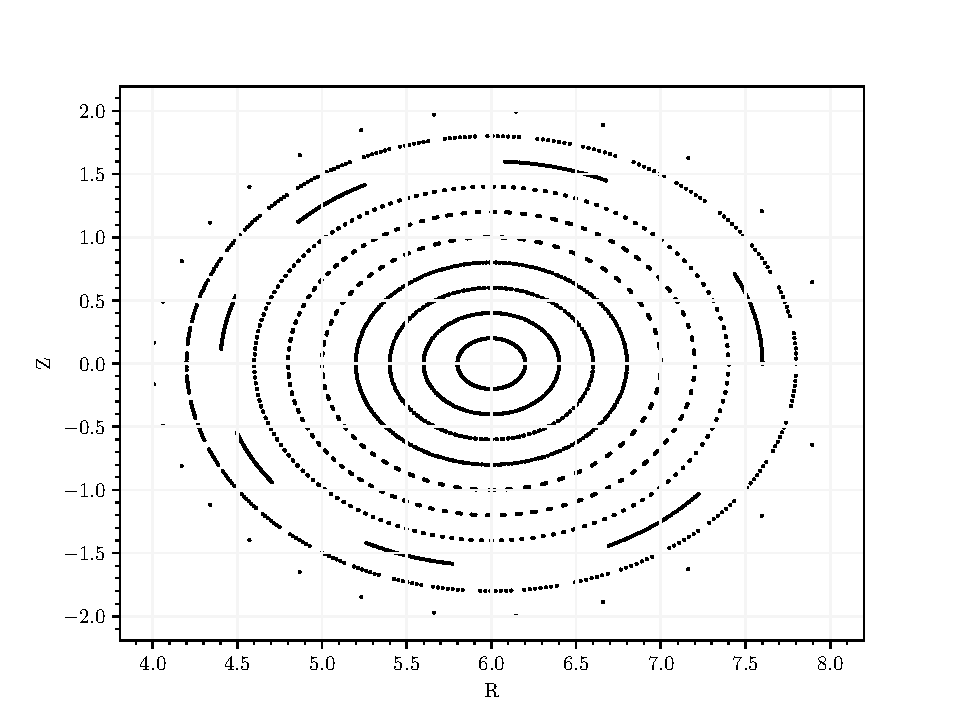
\includegraphics[width=0.5\textwidth]{images/plots/squared-profile/poincare.pdf}
    }
    \hfill
    \subfloat[First sub-figure]{%
        \label{fig:basis-qprofile}
        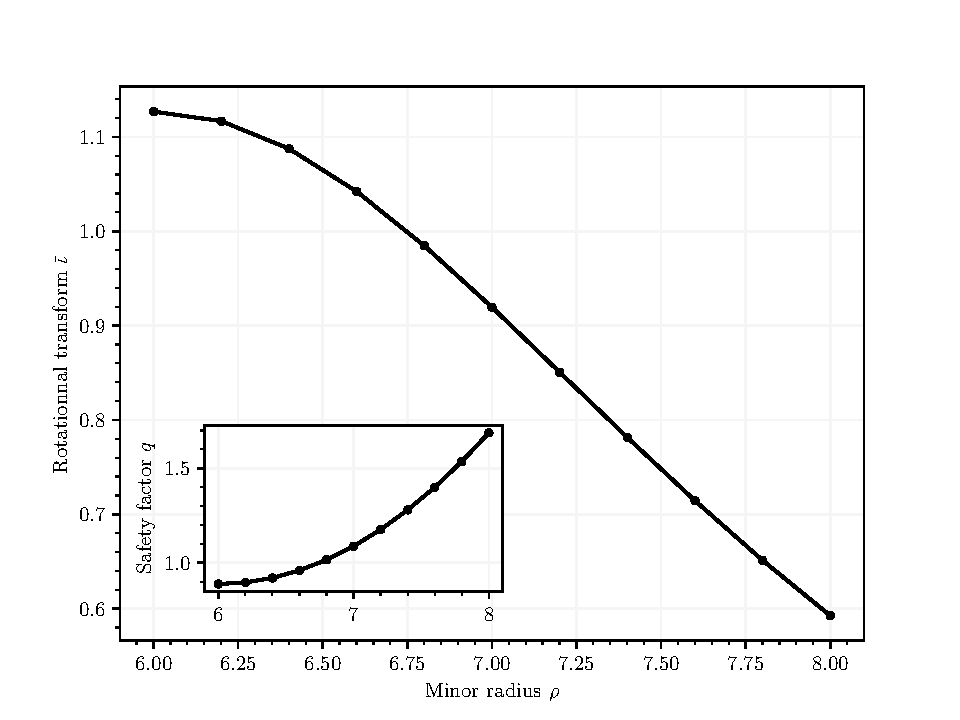
\includegraphics[width=0.5\textwidth]{images/plots/squared-profile/q-iota-squared.pdf}
    }
    \caption{[figure without perturbations]}
\end{figure}

The helicity of a field line can be interpreted as the number of times it wraps around another one. By following of both the magnetic axis as well as the starting point, the helicity $\iotaslash = 1/q$ can be computed by integrating the angle evolution. Performing such a calculation for starting points of the form $(R_0+\rho,0)$ with increasing $\rho$ gives $\iotaslash$ which is represented in \figref{fig:basis-qprofile}. The calculated $q$-profile is in great agreement with its analytical form, which is reasuring.

An essential feature of the diverted tokamak edge structure is the separatrix. Combining a quadratic $q$ equilibrium with the field generated by a circular current loop at appropriate position and amplitude will result in a single null equilibrium. The vector potential of a loop at position $(R_l, 0)$ is given in \cite{simpson_simple_2001} as~:
\begin{align*}
    A^\phi = \frac{\mu_0}{4\pi}\frac{4IR_l}{\beta R}\left(\frac{(2-k^2)K(k^2)-2E(k^2)}{k^2}\right).
\end{align*}
with $K, E$ the complete elliptic integral of the first and second kind and with $\alpha^2 = (R_l-R)^2 + Z^2$, $\beta^2 = (R_l+R)^2+Z^2$ and $k = 1 - \alpha^2/\beta^2$. To get a general position, replace $Z \mapsto Z-Z_l$.

\begin{figure}[h!]
    \begin{minipage}{0.5\textwidth}
        \subfloat[First sub-figure]{%
            \label{fig:toytok-eq}
            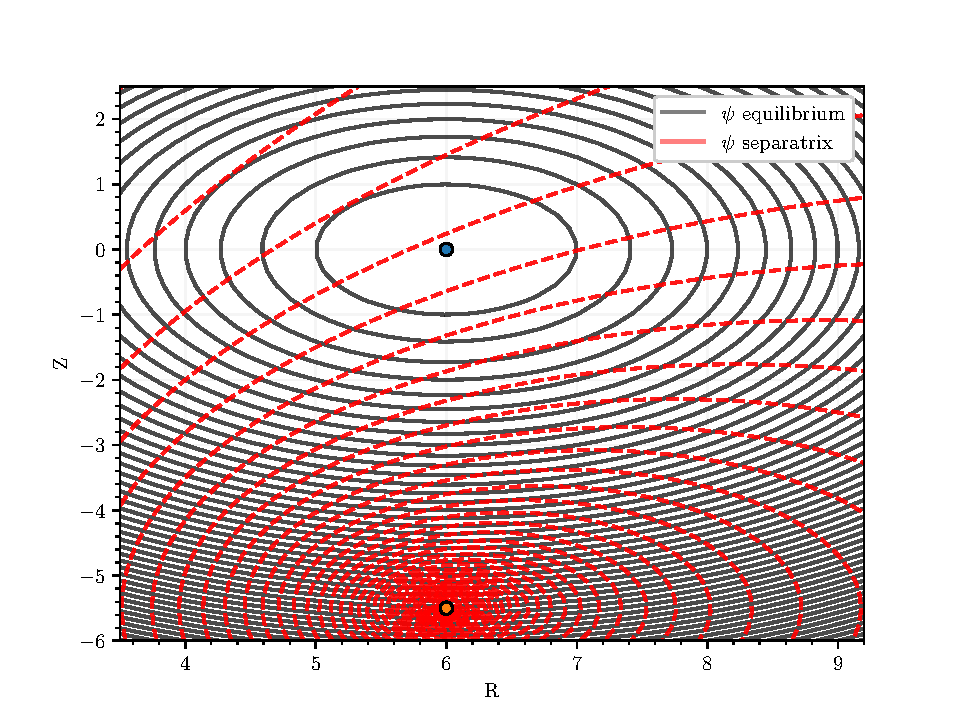
\includegraphics[width=\textwidth]{images/plots/toytok/sepflux.pdf}
        }
        \hfill
        \subfloat[Second sub-figure]{%
            \label{fig:toytok-qprofile}
            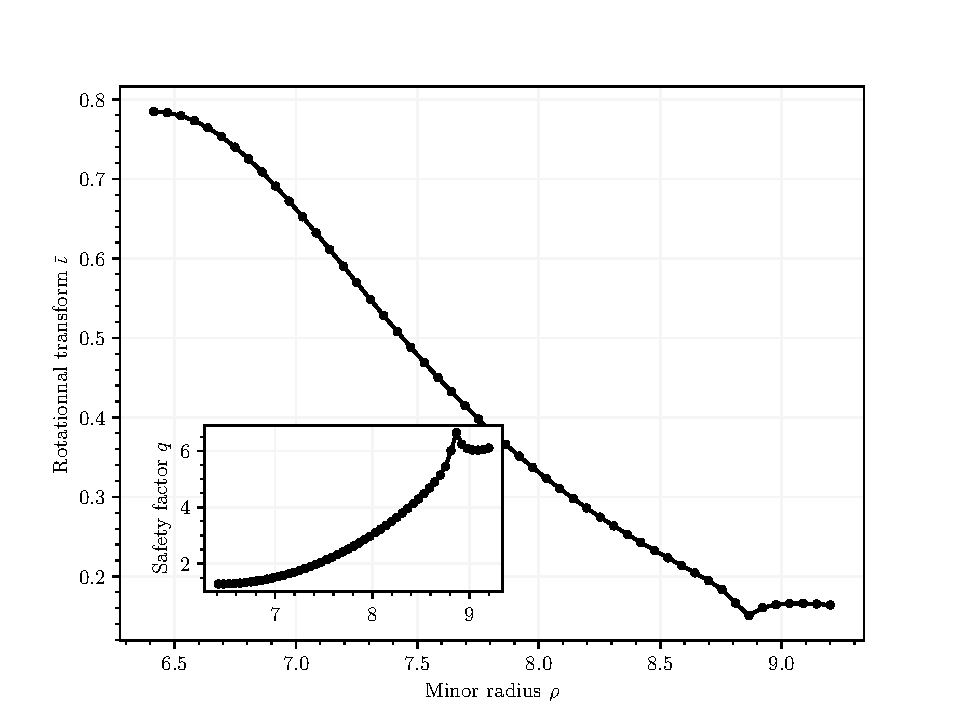
\includegraphics[width=\textwidth]{images/plots/toytok/q-iota-squared.pdf}
        }
    \end{minipage}
    \begin{minipage}{0.5\textwidth}
        \subfloat[Third sub-figure]{%
            \label{fig:toytok-poincare}
            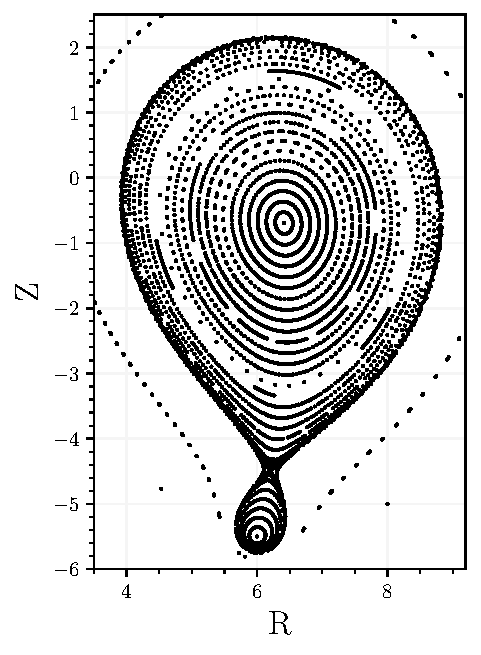
\includegraphics[width=\textwidth]{images/plots/toytok/poincare.pdf}
        }
    \end{minipage}
    \caption{Figure without perturbations}
    \label{fig:basis}
\end{figure}

Setting 
$R = 6, Z = 0, q_0 = 0.91, shear 1.2$

\figref{fig:toytok-eq} shows the contour of $\psi_\text{sep}$ on $\psi$.
[comparison with d3d or tcv for the reality of the toybox]

\section{Perturbations}
adding perturbation to create chaos, not axisymmetric anymore.

The perturbations can be added into the straight field line coordinates or as hamiltonian formalism. show there equivalence.

In the toroidal coordinates the $\phi$ and $\theta$ angles are both $\in [0, 2\pi)$ with $R_\text{max}(\theta)$ and thus one can develop any component into Fourier series as for the magnetic vector potential $\textbf{A}$.
\begin{align*}
    A^i(\rho,\phi,\theta) = \sum\limits_{n\in\mathbb{N}}\sum\limits_{m\in\mathbb{N}} A^i(\rho)\cos(n\phi + \varphi_n)\cos(m\theta + \varphi_m)
\end{align*}
One perturbation mode pair $(m,n)$ and remembering that the equilibrium is axisymmetric, thus one can choose the $\phi$ origin such that $\varphi_m = 0$, the perturbation becomes a choice of $\psi(\rho) = f(\rho)$.

Here the two choices~:

\begin{enumerate}
    \item $f(\rho, \mu, \sigma) = \frac{1}{\sqrt{2\pi\sigma^2}}\exp\left(\frac{-(\rho-\mu)^2}{2\sigma^2}\right)$ from the Normal distribution
    
    \item $f(\rho, d) = \frac{\sqrt{2}}{\sqrt{\pi}}\frac{\rho^2}{d^3}\exp\left(\frac{-\rho^2}{2d^2}\right)$ from the Maxwell-Boltzmann distribution
\end{enumerate}

In fact, the transformation to toroidal does not have to be the one of a circle. One can, for instance, find the flux coordinate for a tokamak equilibrium. Here only a generalization to an ellipsoid is implemented~:
\begin{align*}
    \rho &= \sqrt{\left(\frac{R-R_a}{A}\right)^2 + \left(\frac{Z-Z_a}{B}\right)^2}\\
    \phi &= \phi\\
    \theta &= \text{arctan2}(\frac{Z-Z_a}{B}, \frac{R-R_a}{A})\\
\end{align*}

and when straight field line coordinate are defined, one can transform $\theta$ and $\rho$ to be the 


talk about mode mixing : this is an choice in the way we apply the perturbation to mix mode.


\begin{figure}[h!]
    \subfloat[First sub-figure]{%
        \includegraphics[width=0.5\textwidth]{example-image-a}
    }
    \hfill
    \subfloat[First sub-figure]{%
        \includegraphics[width=0.5\textwidth]{example-image-b}
    }
    \caption{3/2 in the high aspect ratio case and 6/1 in the toytok case}
\end{figure}

we can see that they follow the field on the trargeted q for the high aspect and at the separatrix for the toytok. 

however the toroidal coordinates are not the straight field and if we plot at a $\rho = const$ we can see that
\begin{figure}[h!]
    \subfloat[First sub-figure]{%
        \includegraphics[width=0.5\textwidth]{example-image-a}
    }
    \hfill
    \subfloat[First sub-figure]{%
        \includegraphics[width=0.5\textwidth]{example-image-b}
    }
    \caption{mode mixing for the toyHA}
\end{figure}

\begin{figure}[h!]
    \subfloat[First sub-figure]{%
        \includegraphics[width=0.5\textwidth]{example-image-a}
    }
    \hfill
    \subfloat[First sub-figure]{%
        \includegraphics[width=0.5\textwidth]{example-image-b}
    }
    \caption{mode mixing for the toytok}
\end{figure}

mode mixing is good because it create chaos fast, non definition of flux coordinate at the separatrix. The chaos appearing by ramping up the amplitude.

\begin{figure}[h!]
    \subfloat[First sub-figure]{%
        \includegraphics[width=0.5\textwidth]{example-image-a}
    }
    \hfill
    \subfloat[First sub-figure]{%
        \includegraphics[width=0.5\textwidth]{example-image-b}
    }
    \caption{ramping up the amplitude make the chaos appear in the 6/1 case}
\end{figure}

\chapter{Tangles and Turnstile}

when chaos appear the separation of a separatrix when.
KAM theory

tangles for the tokamap, the henon map
we see that there were a separatrix and then they break to give.

the tangles

The jacobian of $\dpmap$ is $\mathcal{P}(x^\star) = x^\star$ fixed points of a discrete dynamical system.

\section{Stable and Unstable Manifolds}

from poincare also called them trellis [cite]
manifold, manifold ordering.

algorithm to plot them, from.

[plot of the manifold, toytok 6-1, toystell 3/2]

laking behind due to the q-profile
the shape first goes out and then comes back.

the tangle structure they create

\section{Hetero/Homo-clinic points}
[floer homology from sonja]
what are they and algorithm to find them

interested in primary homo-hetero clinic points

algorithm to find them on 6/1 and the fact that we need to find another one, say that we can just initialize with lambda being half.

the rosenbruck structure, and the sneaking returns when the amplitude is increased

the fact that we have more than one
higher order homoclinic points
toyha in 3 2 

the idea to initilize with specific epsilon values to have a nice initial guess. The fact that this is the main point were robustness may be increased.

\section{Turnstile}

the definition of a bounded rezonance zone with island inside and a chaotic layer.

the formal definition by Meiss

[FIGURE with evolution entering and exiting sets]

How the conservation of the flux implies that the entering and exiting sets have the same flux.

\subsection{Integration of the action}

The vector potential $\textbf{A} \in T\,\mathbb{R}^3$ is $\textbf{A} =  A^i\partial_i^\text{cyl}$.

$g = dR\otimes dR + R^2\,d\phi\otimes d\phi + dZ\otimes dZ$

The curvilinear integral of the scalar product $\textbf{A}\cdot\textbf{dl}$ along $\gamma$~:
\begin{align*}
    \int_0^\phi g(\textbf{A},\textbf{dl}) = \int_0^\phi g(\textbf{A}(\gamma(s)),\dot{\gamma}(s))ds\\ = \int_0^\phi (A^R\dot{\gamma}^R + R^2A^\phi\dot{\gamma}^\phi + A^Z\dot{\gamma}^Z) ds
\end{align*}
Thus for a $q=m/n=1/0$ fixed point of with $n_\text{fp} = 1$, it gives $2\pi R^2A^\phi = 2\pi R\tilde{A}^\phi$ with $\tilde{A}^\phi$ the $\phi$ component into the usual orthonormal cylindrical basis.

\subsection{algorithm}

the use of stokes theorem, cite Meiss again.
The specific contour

the mapping forward and backward to reduce the lenght and bring them back where there geometry is easy.

then in the linear regime take just segments for gamma 1 and gamma 3 and approximate the integral which takes literally no time.

question ? why not just find the contour with many points and calculate a dot dl ? This is an idea however here we remember that the poincare map is performed by integrating the field and in the latter case of real stellarator geometry it will take long to compute for instance even 100 points in u and s. (200pts * 5 integrations each will give) 1000 necessary integration against only 2 once the homoclinics are found, this allows to use a higher tolerance on the integrator. Note in the case you also need to be sure that your grid is fine enough to have the intersections in it. The complexity is different, here it is used for verification.

actual calculation with the path 

verification with triangle, shoelace and the a dot dl along the contour.